\section{Execution Plan}
\label{executionplan}

The general execution pipeline, in Figure \ref{pipeline}, provides an overview of the steps that will be followed. Hereafter, we will analyse for each research question how the experiment was conducted.
\subsection{\textbf{RQ$_{1}$} - Comparing a standard ViT with Our Proposal} 
After implementing in PyTorch our architecture described in Section \ref{architecture} we are going to train from scratch a ViT and our model and comparing them using the metrics explained in Section \ref{metrics}.

For the energy efficiency analysis we will use CodeCarbon, which provides an accurate estimation of the energy producted by RAM, GPUs and CPUs during the executing of the code (we will use Colab to perform the operations in as isolated an environment as possible \textit{"Intel Xeon @ 2.20GHz and Tesla T4 GPU"}). 

At this stage, the hyper-parameters will be fixed and common between the ViT architecture and our model, as our intention is to demonstrate that with the same configuration using a probabilistic approach, performance does not degrade and energy consumption is reduced.

Here follows the configurations for this phase of research, parameters marked by the \textbf{*} symbol are used in the ViT standard architecture, this configuration has been taken from the ViT-H/14, the current state-of-the-art ViT for Image Classification and Object Detection:

\begin{itemize}
    \item in\_channels*: 3
    \item patch\_size*: 16
    \item emb\_size*: 3072
    \item img\_size*: 224
    \item depth*: 16
    \item top\_k: 196 ($100\%$ of the patches)
    \item heuristic: none
    \item probabilistic: false
    \item prob: 1 (means that the heuristic function will not be applied)
    \item prob\_decay\_rate: 0
    \item batch\_size: 512
    \item learning\_rate: 1e-3
\end{itemize}

Further explaination of the additional hyperparameters can be found in the \textbf{RQ$_{2}$} execution plan.

We will perform a statistical validity test with null hypothesis stating that the sample (electric energy consumed repeating the same experiment) follows a normal PDF and alternative hypothesis stating that it does not come from that distribution:
\begin{itemize}
    \item We will perform the Shapiro-Wilk test with significance level 0.05 in the hope of validating the null hypothesis 
    \item If the tests confirm the null hypothesis, then the energy values we will report will be the average of the calculated values.
    \item Finally, we will calculate the Carbon Intensity, which is the grams of CO$_2$ produced by running the code as the product of the Net Carbon Intensity (A weighted average of the emissions from the different energy sources that are used to generate electricity consumed by the Cloud provider or Country) and the KWh consumed.
\end{itemize}

\subsection{\textbf{RQ$_{2}$} - In Search of Heuristic that lead to a faster convergence}
When a human being is asked to understand an object represented on an image, a logical process is generally carried out that leads to discarding all information that does not concern the object itself. Based on this theory, we will implement a feature selection layer based on three different heuristics.
Given that every patch in which the image is divided is an $n \times n$ matrix the value of each patch $x$ is calculated as follows:
\begin{itemize}
    \item Contrast (Figure \ref{fig:dog_contrast}):  $$F(x) =  \frac{max(x) - min(x) + 10^{-8}}{max(x) + min(x)}$$ 
   
    \item Variance (Figure \ref{fig:dog_variance}): $$F(x) =  \frac{\sum_{i=1}^n\left(x_i-\overline{\mathbf{x}}\right)^2}{n-1}$$
       
    \item Entropy (Figure \ref{fig:dog_entropy}): $$F(x) =  -\sum_{i=1}^{n}(p_i * log2(p_i))$$\\ where $$p_i = \frac{count(i)}{N}$$
        
\end{itemize}
    \begin{figure}[!htp]
        \centering
        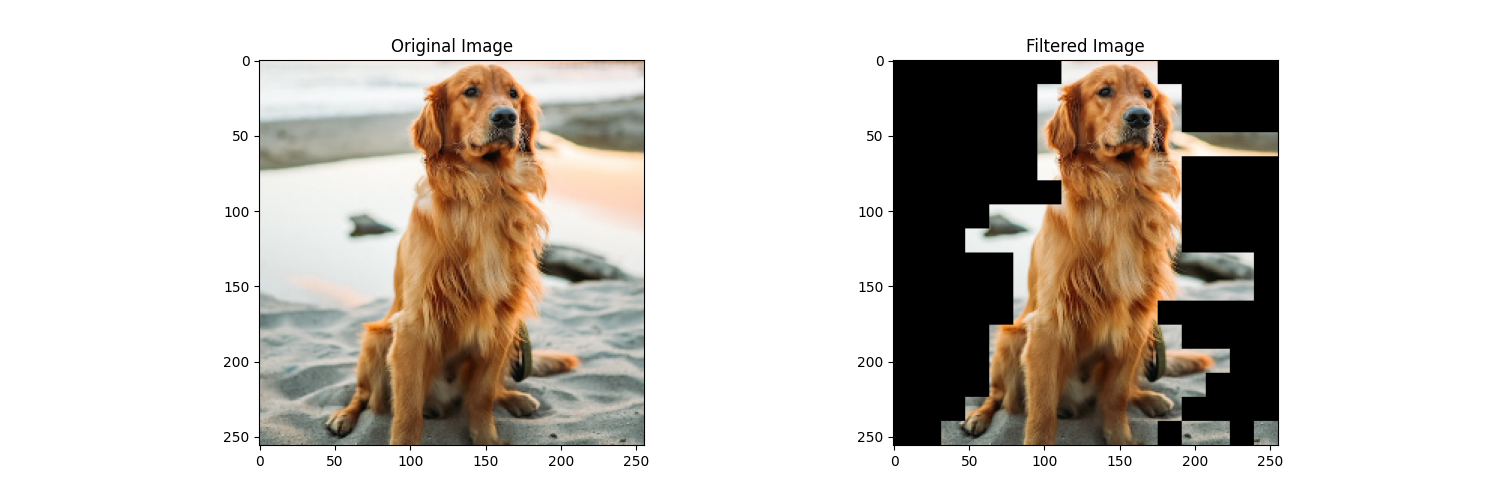
\includegraphics[width=\columnwidth]{images/dog_contrast.png}
        \caption{Image filtered based on contrast values distribution preserving 50\% of image}
        \label{fig:dog_contrast}
    \end{figure}
     \begin{figure}[!htp]
        \centering
        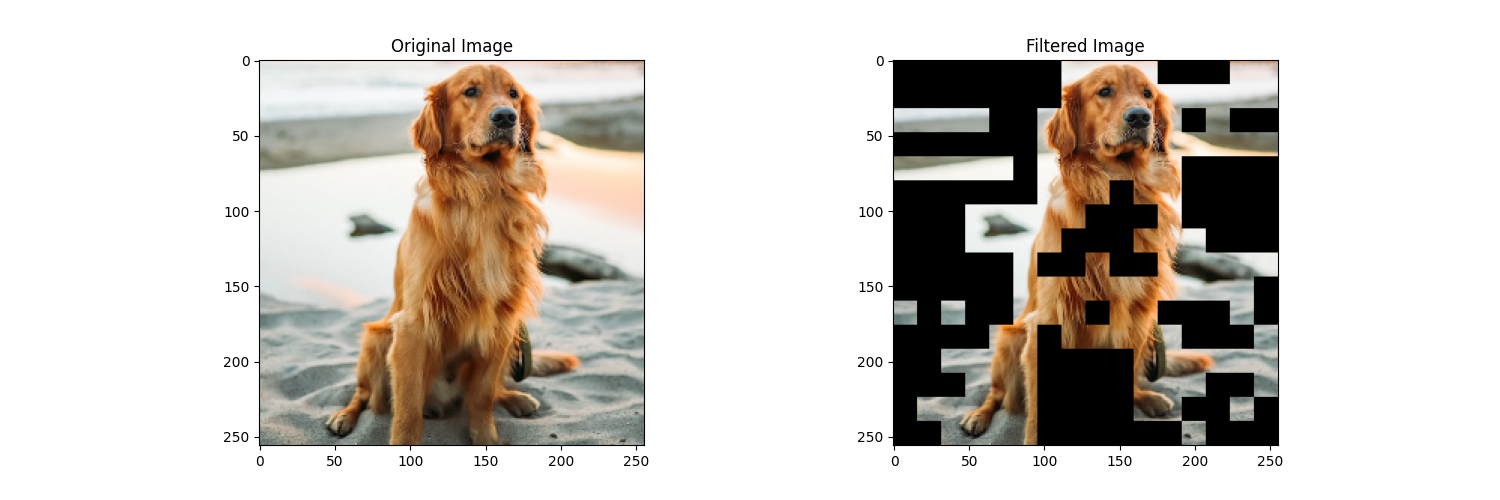
\includegraphics[width=\columnwidth]{images/dog_variance.png}
        \caption{Image filtered based on variance values distribution preserving 50\% of image}
        \label{fig:dog_variance}
    \end{figure}
    \begin{figure}[!htp]
        \centering
        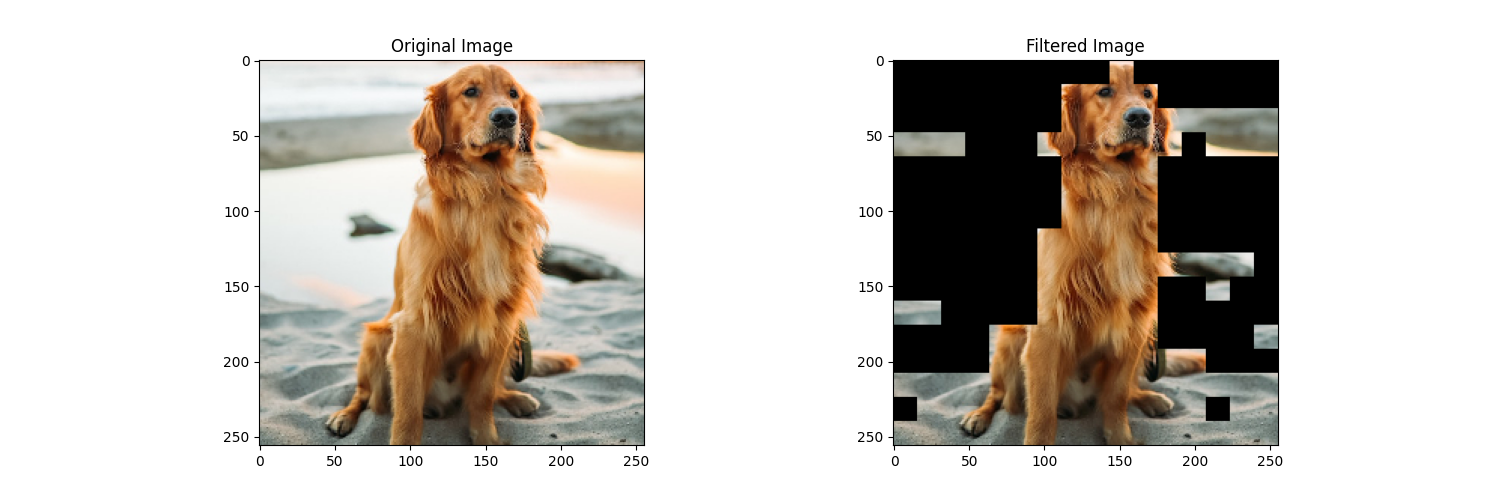
\includegraphics[width=\columnwidth]{images/dog_entropy.png}
        \caption{Image filtered based on entropy values distribution preserving 50\% of image}
        \label{fig:dog_entropy}
    \end{figure}
    
We are going to perform the experiments on different hyperparameters, keeping fixed the learning rate fixed at $1e-3$, showed in Table \ref{tab:hyperparameters}, parameters marked by the \textbf{*} symbol are used in the ViT standard architecture counterpart.
\begin{table*}[!htp]
\centering
\begin{tabular}{|l|ccc|ccc|ccc|}
\multicolumn{1}{l}{\textbf{}} & \multicolumn{1}{l}{\textbf{}} & \multicolumn{1}{l}{\textbf{4 heads}} & \multicolumn{1}{l}{\textbf{}} & \multicolumn{1}{l}{\textbf{}} & \multicolumn{1}{l}{\textbf{8 heads}} & \multicolumn{1}{l}{\textbf{}} & \multicolumn{1}{l}{\textbf{}} & \multicolumn{1}{l}{\textbf{12 heads}} & \multicolumn{1}{l}{\textbf{}} \\ \hline
\textbf{in\_channels*}      & 3                             & 3                                    & 3                             & 3                             & 3                                    & 3                             & 3                             & 3                                     & 3                             \\ \hline
\textbf{patch\_size*}       & 16                            & 16                                   & 16                            & 16                            & 16                                   & 16                            & 16                            & 16                                    & 16                            \\ \hline
\textbf{emb\_size*}         & 64                            & 64                                   & 64                            & 64                            & 64                                   & 64                            & 64                            & 64                                    & 64                            \\ \hline
\textbf{img\_size*}         & 224                           & 224                                  & 224                           & 224                           & 224                                  & 224                           & 224                           & 224                                   & 224                           \\ \hline
\textbf{depth*}             & 4                             & 4                                    & 4                             & 8                             & 8                                    & 8                             & 12                            & 12                                    & 12                            \\ \hline
\textbf{top\_k}            & 138                           & 138                                  & 138                           & 138                           & 138                                  & 138                           & 138                           & 138                                   & 138                           \\ \hline
\textbf{heuristic}         & \textit{contrast}             & \textit{variance}                    & \textit{entropy}              & \textit{contrast}             & \textit{variance}                    & \textit{entropy}              & \textit{contrast}             & \textit{variance}                     & \textit{entropy}              \\ \hline
\textbf{probabilistic}     & \textit{true}                 & \textit{true}                        & \textit{true}                 & \textit{true}                 & \textit{true}                        & \textit{true}                 & \textit{true}                 & \textit{true}                         & \textit{true}                 \\ \hline
\textbf{prob}              & 0.5                           & 0.5                                  & 0.5                           & 0.5                           & 0.5                                  & 0.5                           & 0.5                           & 0.5                                   & 0.5                           \\ \hline
\textbf{prob\_decay\_rate} & 5e-3                          & 5e-3                                 & 5e-3                          & 5e-3                          & 5e-3                                 & 5e-3                          & 5e-3                          & 5e-3                                  & 5e-3                          \\ \hline
\textbf{batch\_size}       & 512                           & 512                                  & 512                           & 512                           & 512                                  & 512                           & 512                           & 512                                   & 512                           \\ \hline
\end{tabular}
\caption{RQ$_{2}$ table of hyperparameters}
\label{tab:hyperparameters}
\end{table*}
\begin{itemize}
    \item in\_channels: refers to the number of channel of the image, 1 if gray scale, 3 if rgb
    \item patch\_size: is the size of each $n \times n$ patch into which the image will be divided
    \item emb\_size: the number of dimensions in the feature representation used to encode each patch or region of the image
    \item img\_size: is the size in which the image will be resized
    \item depth: is the number of head of the multi-head attention layer
    \item top\_k: is the number of patches to preserve (e.g $138$ for $224 \times 224$ is equivalent to preserve the $70\%$ of the $196$ patches in which the image will be divided)
    \item heuristic: is the heuristic method that will be used to select the patches
    \item probabilistic: if true the values of each patches will be interpreted as a PDF, otherwise they will be sorted descending
    \item prob: is the probability to chose to use the patches selected or the full image
    \item prob\_decay\_rate: is the decay rate over epoch for the prob hyperparameter in order to use the full image with the succession of epochs
    \item batch\_size: refers to the number of samples or data points processed at a time
\end{itemize}


\subsection{\textbf{RQ$_{3}$} - Assessing the Performance of Our Model on different training technique} In this phase we will train our model using two different techniques

1) Pre-training + Fine-tuning

2) Pre-training + Contrastive Learning + Fine-tuning
\\
Each phase will be executed as follows:
\begin{itemize}
    \item Pre-training: the model will be trained on a large amount of unlabeled data to learn general features. In our pre-training, the model is trained on Tiny ImageNet using a self-supervised task called 'masked language modeling.' This involves randomly masking $15\%$ of patches of the input image and then training the model to predict the masked patches. This way, the model learns to represent the image in terms of meaningful patches of varying sizes and positions.

    \item Contrastive Learning: after pre-training, the model will be further fine-tuned using contrastive learning, which is a form of self-supervised learning. In contrastive learning, the model learns to distinguish between similar and dissimilar image by projecting them into a high-dimensional space and comparing their distances. This way, the model learns to identify patterns and features that are relevant for the downstream task, such as image recognition.
    Positive pair will be similar images.
    Negative pari will be an image randomly selected from a different class.

    \item Fine-tuning : once the model has been pre-trained and fine-tuned with contrastive learning, it will be further fine-tuned on image recognition task on CIFAR-10/CIFAR-100 and object detection on Tiny ImageNet. During fine-tuning, the model is trained on labeled data with a supervised learning approach. In this phase, the last few layers of the model are replaced with new ones, and only the newly added layers are trained on the specific task, while the earlier layers are frozen to retain the learned features. This way, the model can adapt to the specific dataset and learn to recognize the relevant features for the task at hand.
\end{itemize}